\documentclass[11pt]{article}
\usepackage[top=0.7in,bottom=0.7in,left=1in,right=1in]{geometry}
\setlength{\parskip}{1ex plus 0.5ex minus 0.2ex}

\usepackage{amsmath}
\usepackage{amsfonts}
\usepackage{graphicx}
\usepackage[colorlinks=true,citecolor=red,linkcolor=blue]{hyperref}
\usepackage[]{natbib}

\graphicspath{{figs/}}

\usepackage{lineno}
%\linenumbers

\renewcommand{\vec}[1]{\boldsymbol{#1}}
\newcommand{\uvec}[1]{\hat{\boldsymbol{#1}}}
\newcommand{\mat}[1]{\boldsymbol{#1}}

\newcommand{\rmax}{r_c}

\newcommand{\suprcv}[1]{#1^{\mathrm{rcv}}}
\newcommand{\suplcl}[1]{#1^{\mathrm{lcl}}}

\begin{document}
\sloppy

\begin{center}
{\bf A method and software to calculate stress on a curved elastic dislocation} \\
\vspace{1em}
Andrew M.~Bradley\footnote{Andrew M.~Bradley (andrew.bradley@gmail.com)} \\
\end{center}

\begin{abstract}
This document describes the theory implemented in the open-source library Woodland \citep{woodland-software}.
The Displacement Discontinuity Method (DDM)
is a type of Boundary Element Method designed to model elastic fracture mechanics efficiently.
The DDM discretizes a fracture, for example a fault in Earth's crust.
It relates dislocation, or displacement discontinuity,
on the elements in the discretization to stress on the elements.
The key calculation in forming a DDM discretization is the interaction integral,
and the self-interaction integral is particularly challenging.
Historically, most DDM discretizations have treated uniformly gridded, mathematically one-dimensional, flat fractures.
More recently, two-dimensional (2D), usually uniformly gridded and flat fractures in a three-dimensional (3D) space have been studied.
Generally curved, 2D, nonuniformly gridded fractures in a 3D space remain a challenge for two reasons.
First, flat elements with constant dislocation,
which are almost always used in studies,
do not generally provide a convergent approximation in this fully general case.
Second, curved elements make the self-interaction integral difficult to compute.
This document describes a numerical method to approximate the self-interaction integral for
smooth dislocation over a smooth, curved 2D element in a 3D space,
which we term the \emph{circular-sector finite-part} (CSFP) method.
Numerical results compare application of a discretization using the CSFP method
with a standard reference discretization
as well as with other discretizations of interest.
Discretizations using the CSFP method achieve high-order convergence.
It is demonstrated that both curved elements and high-order approximation of dislocation
are necessary in general.
\end{abstract}

\section{Introduction}

The Displacement Discontinuity Method (DDM) \citep{crouch1983boundary}
is a type of Boundary Element Method designed to model elastic fracture mechanics efficiently.
The DDM discretization relates dislocation, also known as displacement discontinuity, to stress over a fracture surface.
This linear operator is an important component in quasi-dynamic earthquake simulators
(\citep{rice1993spatio}; recently, \citep{ozawa2023large,herrera2024seismic})
and usually the most computationally demanding part of a simulator,
both to form and to apply.
The DDM discretization is most often of the collocation type,
computing stress at each collocation point due to dislocation at all collocation points.

The key calculation in constructing the collocation DDM discretization is the \emph{interaction integral}
that relates dislocation over one element to stress at a point on the fracture,
including within the element.
Existing methods include
the fast Fourier transform \citep[e.g.][Ch.~4]{segall2010earthquake} for uniform elements on a flat fracture with constant dislocation within each element;
flat general elements with constant dislocation over the element \citep{okada1992internal,meade2007algorithms,gimbutas2012calculation,barall2016performance};
and flat general elements with high-order dislocation \citep{shou1995higher,meade2022bem2d}.
Each method is combined with
a specification of the element grid
and the basis functions and degrees of freedom on that grid
to form a discretization of the elasticity problem.
These methods to compute the interaction integral are suited for collocation discretizations.
\citet{thompson2019boundary} describe a Galerkin method.
More work should be done to compare and contrast collocation and Galerkin methods in DDMs.

In the most general case of a curved fracture,
it is not sufficient to use flat elements in the collocation DDM discretization,
as we demonstrate in this document.
Thus, we describe a numerical method to
compute the interaction integral relating high-order dislocation over a curved element to stress on the curved fracture.
This numerical method can be used to construct a variety of discretizations.
This method is implemented in the open-source library Woodland \citep{woodland-software},
and this document is the theory manual for that software.

None of what follows is particularly original.
The methods are classical.
The approach to computing the Hadamard finite part over an element is most similar to ideas described in \citet{guiggiani1998formulation}.
Other references with detailed treatments of similar calculations include \citet{kanduvc2022isoparametric} and \citet{peng2017isogeometric}.

This document is structured as follows.
Section~\ref{sec:methods} describes the interaction integral and a numerical method to compute it.
Section~\ref{sec:results} demonstrates the method
and compares numerical results from several discretizations.
Finally, Sec.~\ref{sec:conclusions} concludes.

\section{Computing the interaction integrals} \label{sec:methods}

To derive the homogeneous, isotropic, full-space elastic stress tensor \eqref{eq:stress},
we follow \citet{okada1992internal} and \citet{gimbutas2012calculation}.
% src y, obs x
% deriv wrt x or y gives same
% Lame coefficients:
%   alpha = (lambda + mu)/(lambda + 2 mu)
%   lambda = 2 mu nu/(1 - 2 nu)
%   nu = lambda/[2 (lambda + mu)]
% check against Segall 3.91:
%   a = (l + u)/(l + 2 u)
%   v = l/[2 (l + u)]
%   1/[4 (1 - v)]
%     = 1/[4 (1 - l/[2 (l + u)])]
%     = 2 (l + u)/[4 (2 (l + u) - l)]
%     = 2/4 (l + u)/(l + 2 u)
%     = a/2
The displacement at $\vec{x}$ in the $i$ direction
due to a unit point force at $\vec{y}$ in the $j$ direction is
given by the Kelvin solution,
\begin{linenomath}\begin{equation*}
  U_i^j = \frac{1}{4 \pi \mu} \left( \frac{\delta_{ij}}{R} -
         \frac{\alpha}{2} \frac{\partial}{\partial y_i} \frac{\partial}{\partial y_j} R \right),
\end{equation*}\end{linenomath}
where $\alpha = (\lambda + \mu)/(\lambda + 2 \mu)$,
$\lambda$ and $\mu$ are the Lam\'{e} coefficients,
and $R = \sqrt{\sum_{i=1}^3 (x_i - y_i)^2}$.
%
In terms of $U_i^j$, the displacement at $\vec{x}$ in the $i$ direction
due to a unit dislocation in the $j$ direction
on a surface having unit normal in the $k$ direction is
\begin{linenomath}\begin{equation*}
  T_{ik}^j = \lambda \delta_{jk} \frac{U_i^n}{\partial y_n} +
            \mu \left( \frac{U_i^j}{\partial y_k} + \frac{U_i^k}{\partial y_j} \right).
\end{equation*}\end{linenomath}
For a dislocation vector $\vec{d}$
on a surface having normal vector $\uvec{n}$,
the displacement is
\begin{linenomath}\begin{equation*}
  u_i(\vec{x}, \vec{y}, \uvec{n}, \vec{d}) = T_{ik}^j n_k d_j,
\end{equation*}\end{linenomath}
and the stress tensor is
\begin{equation} \label{eq:stress}
  \sigma_{ij}(\vec{x}, \vec{y}, \uvec{n}, \vec{d})
    = \lambda \delta_{ij} \frac{\partial u_n}{\partial x_n} +
      \mu \left( \frac{\partial u_i}{\partial x_j} + \frac{\partial u_j}{\partial x_i} \right).
\end{equation}
This expression is the \emph{point Green's function}
for the elastic full-space problem.
The interaction integral requires integrating the point Green's function over an element
to form the \emph{element Green's function}.

\begin{figure}[tb]
  \centering
  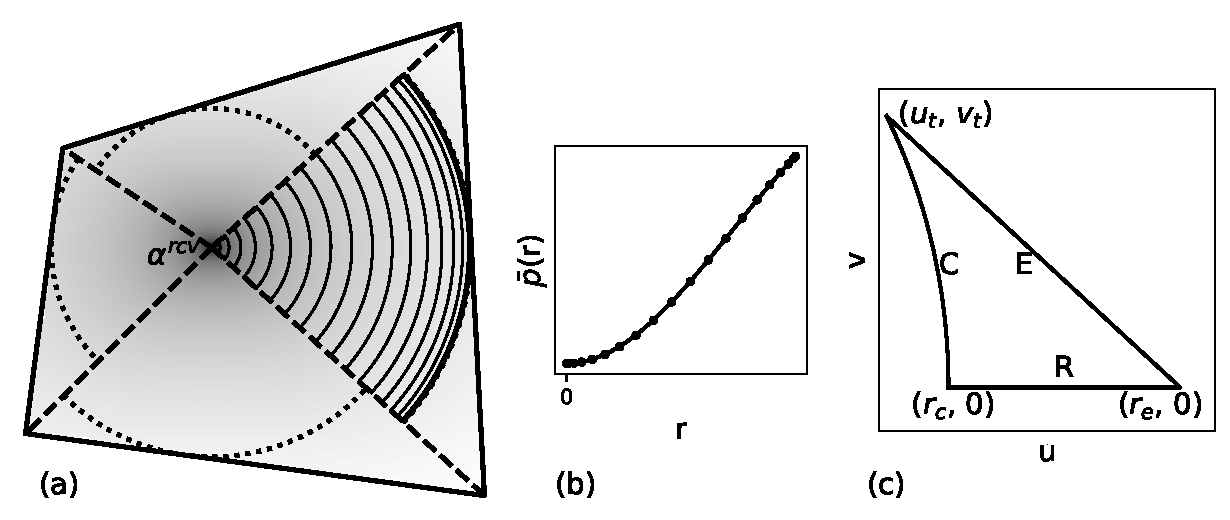
\includegraphics[width=1\linewidth]{schematic-self-interaction}
  \caption{(a) A parameter polygon and its decomposition.
  Bold lines outline the polygon, a quadrilateral.
  The receiver point, $\suprcv{\vec{\alpha}}$,
  is at the intersection of the four circular sectors.
  Circular segments fill the right circular sector;
  dotted curves indicate three other circular sectors.
  The shaded background is the logarithm of the singular integrand.
  (b) The function $\bar{p}(r)$ associated with the right circular sector.
  (c) A CR triangle in local coordinates $(u,v)$.}
  \label{fig:diagram}
\end{figure}

In this document, an element on a fracture in three dimensions is parameterized by a map
between a flat, straight-sided \emph{parameter} polygon in a convenient coordinate system and the
generally curved but smooth \emph{physical} element,
with both curved edges and interior surface.
Let $\vec{\alpha} \in \Omega \subset \mathbb{R}^2$
be the parameters of the parameter polygon $\Omega$,
and let $\vec{y}(\vec{\alpha}): \mathbb{R}^2 \rightarrow \mathbb{R}^3$,
$\vec{\alpha} \in \Omega$,
be a smooth, nonsingular map between the parameter polygon and the physical element.
A simple example is a parameterized surface $(x, y, z(x,y)) \in \mathbb{R}^3$.
In this example, a parameter polygon is a polygon
$\vec{\alpha} \equiv (x,y) \in \Omega \subset \mathbb{R}^2$.
The physical element is the image of $\Omega$ on the parameterized surface $z(x,y)$,
and $\vec{y}(\vec{\alpha}) \equiv (x, y, z(x,y))$.

Consider the receiver point
$\vec{x} = \vec{y}(\suprcv{\vec{\alpha}})$ for $\suprcv{\vec{\alpha}} \in \Omega$.
Figure \ref{fig:diagram}(a) illustrates these and other quantities.
The stress at $\vec{x}$ due to dislocation over the element is the interaction integral
\begin{equation} \label{eq:main}
  \sigma_{ij}^\mathrm{rcv}(\vec{x}; \Omega) =
  \mathrm{f.p.} \int_\Omega
    \sigma_{ij}(\vec{x}, \vec{y}(\vec{\alpha}), \uvec{n}(\vec{\alpha}), \vec{d}(\vec{\alpha})) \
    \sqrt{\mathrm{det}(\vec{y}_{\vec{\alpha}}(\vec{\alpha})^T \vec{y}_{\vec{\alpha}}(\vec{\alpha}))} \
    \mathrm{d} \vec{\alpha},
\end{equation}
where $\vec{y}_{\vec{\alpha}}(\vec{\alpha})$ is
the 3$\times$2 Jacobian matrix.
Because $\suprcv{\vec{\alpha}} \in \Omega$,
the integrand has the singularity $\|\vec{y}(\vec{\alpha}) - \vec{x}\|^{-3}$;
thus, we require the Hadamard finite part (f.p.)~of the integral.
If $\suprcv{\vec{\alpha}} \notin \Omega$,
then \eqref{eq:main} is a proper integral.
Because the finite part of a proper integral is just the integral,
\eqref{eq:main} describes the interaction integral in all cases.

If $\suprcv{\vec{\alpha}} \notin \Omega$
and is not too close to $\Omega$,
then \eqref{eq:main} can be approximated by
standard tensor and triangular \citep[e.g.][]{Dunavant1985,Taylor2007,Zhang2009} quadrature methods,
usually by first decomposing the polygon $\Omega$ into subtriangles.
We refer to this case as the \emph{other-interaction integral}.
If $\suprcv{\vec{\alpha}}$ is on the boundary of $\Omega$,
$\sigma_{ij}(\vec{x},\Omega)$ can be singular;
if it is near the boundary, it can be nearly singular.
In a discretization having sufficient smoothness,
this type of singularity is canceled by adjacent elements;
however, exploiting this cancellation couples adjacent elements,
adding complexity to the discretization.
Because it is not hard to design a collocation discretization so that
no receiver point is near a boundary,
we assume $\suprcv{\vec{\alpha}}$ is not on or near the boundary of $\Omega$.

Now we consider the case $\suprcv{\vec{\alpha}} \in \Omega$
and not near a boundary.
We refer to this case as the \emph{self-interaction integral}.
If the element is flat,
then Green's theorem can be used to transform
the surface hypersingular integral \eqref{eq:main} into
a proper integral over the boundary of $\Omega$.
This method is used in the derivation of most, if not all,
closed-form interaction integrals for flat elements.
\citet{gimbutas2012calculation} describe this approach
in the case of constant dislocation,
and the method generalizes to high-order dislocation.
If the element is curved,
while we will not attempt to prove that Green's theorem in general will no longer work,
we expect that it will not.
We now describe a numerical method for this latter case.

To introduce the method,
first consider a flat element with constant dislocation.
Then the integrand in \eqref{eq:main} reduces to
$g(\theta)/r^3$,
where the receiver $\suprcv{\vec{\alpha}}$ is at radial coordinate $r = 0$
and $g(\theta)$ is a smooth, nonsingular function of only the angular coordinate $\theta$.
Consider a circular sector $\omega \subset \Omega$
having center $\suprcv{\vec{\alpha}}$,
radius $\rmax$,
and angular extent $[\theta_1,\theta_2]$.
Figure \ref{fig:diagram}(a) shows four circular sectors.
The integral over just the circular sector $\omega$ is
\begin{linenomath}\begin{align}
  \sigma_{ij}^\mathrm{rcv}(\vec{x}; \omega) &=
    \mathrm{f.p.} \int_0^{\rmax} \int_{\theta_1}^{\theta_2}
    \frac{g(\theta)}{r^3} \
    r \ \mathrm{d} \theta \mathrm{d} r \notag \\
  &= \mathrm{f.p.} \int_0^{\rmax} \frac{1}{r^2}
     \int_{\theta_1}^{\theta_2} g(\theta) \ \mathrm{d} \theta \mathrm{d} r \notag \\
  &= G(\theta_1,\theta_2) \ \mathrm{f.p.} \int_0^{\rmax} \frac{1}{r^2} \ \mathrm{d} r \notag \\
  &= -\frac{G(\theta_1,\theta_2)}{\rmax}, \label{eq:flatconst-case}
\end{align}\end{linenomath}
where $G(\theta_1,\theta_2)$ is a smooth, nonsingular function.

Next, consider the general case of a curved element and high-order dislocation.
We use the map $\vec{\alpha}(r,\theta)$ from radial coordinates $(r,\theta)$ to the parameters $\vec{\alpha}$.
The integral over the circular sector $\omega$ is
\begin{equation} \label{eq:general-integral}
  \sigma_{ij}^\mathrm{rcv}(\vec{x}; \omega) =
  \mathrm{f.p.} \int_0^{\rmax} \int_{\theta_1}^{\theta_2}
    \sigma_{ij}(\vec{x}, \vec{y}(\vec{\alpha}), \uvec{n}(\vec{\alpha}), \vec{d}(\vec{\alpha})) \
    \sqrt{\mathrm{det}(\vec{y}_{\vec{\alpha}}(\vec{\alpha})^T \vec{y}_{\vec{\alpha}}(\vec{\alpha}))} \
    | \mathrm{det}(\vec{\alpha}_{(r,\theta)}) | \
    \mathrm{d} \theta \mathrm{d} r.
\end{equation}
Write this integral as
\begin{linenomath}\begin{align}
  \sigma_{ij}^\mathrm{rcv}(\vec{x}; \omega) &=
  \mathrm{f.p.} \int_0^{\rmax} \int_{\theta_1}^{\theta_2}
    \frac{f(r,\theta)}{r^3} \
    r \ \mathrm{d} \theta \mathrm{d} r \notag \\
  &= \mathrm{f.p.} \int_0^{\rmax} \frac{1}{r^2}
    \int_{\theta_1}^{\theta_2} f(r,\theta) \ \mathrm{d} \theta
    \mathrm{d} r \notag \\
  &= \mathrm{f.p.} \int_0^{\rmax} \frac{F(r,\theta_1,\theta_2)}{r^2} \
    \mathrm{d} r, \label{eq:general-case}
\end{align}\end{linenomath}
where $f(r,\theta)$ is a smooth, nonsingular function of both the radial and angular coordinates.
In the final line, let $p(r) \equiv F(r,\theta_1,\theta_2)$.

If the element is flat,
then only the high-order dislocation makes $p(r)$ deviate from a constant.
High-order dislocation affects \eqref{eq:main} only through $\vec{d}$ in \eqref{eq:stress};
in particular, the area element is still constant.
Thus, we can expect typical basis functions used in the representation of dislocation
to lead to a closed-form finite part in \eqref{eq:general-case}.
In contrast, element curvature affects $\vec{y}$ and, thus, $\vec{y}_{\vec{\alpha}}(\vec{\alpha})$,
fundamentally altering the integrand in \eqref{eq:main},
including the area element.

However, the form of $p(r)$ makes a numerical approximation possible.
Because $f(r,\theta)$ is smooth and nonsingular,
we can decompose $p(r)$ as
\begin{linenomath}\begin{equation*}
  p(r) = p(0) + p_r(0) r + (p(r) - p(0) - p_r(0) r),
\end{equation*}\end{linenomath}
where
\begin{linenomath}\begin{equation} \label{eq:Or2}
  p(r) - p(0) - p_r(0) r = \sum_{n=2}^{\infty} \frac{p^{(n)}(r)}{n!} r^n
\end{equation}\end{linenomath}
at and near $r=0$, and $p^{(n)}(r)$ is the $n$th derivative of $p(r)$.
Then
\begin{linenomath}\begin{align}
  \sigma_{ij}^\mathrm{rcv}(\vec{x}; \omega)
  &= \mathrm{f.p.} \int_0^{\rmax}
    \frac{p(r)}{r^2} \
    \mathrm{d} r \notag \\
  &= \mathrm{f.p.} \int_0^{\rmax}
    \frac{p(0)}{r^2} + \frac{p_r(0)}{r} + \frac{p(r) - p(0) - p_r(r) r}{r^2} \
    \mathrm{d} r \notag \\
  &= -\frac{p(0)}{\rmax} + p_r(0) \log \rmax +
    \int_0^{\rmax} \frac{p(r) - p(0) - p_r(r) r}{r^2} \ \mathrm{d} r. \label{eq:circsec}
\end{align}\end{linenomath}
The third term in \eqref{eq:circsec} is a proper integral due to \eqref{eq:Or2}.
The derivation of \eqref{eq:circsec} uses a classical technique called
\emph{singularity subtraction} \citep[e.g.][]{davis2007methods,klockner2013quadrature,kanduvc2022isoparametric}:
isolate the singularity in one or more terms whose finite parts can be calculated in closed form,
then treat the remaining proper integral.

In the case of constant dislocation over a flat element, $p(r)$ is constant in $r$,
as the derivation of \eqref{eq:flatconst-case} shows.
In the general case of smooth dislocation over a smoothly curved element,
it is a smooth function.
We do not have direct access to $p(r)$
because its value at each $r$ is a function of an integral in the angular coordinate $\theta$.
But we can approximate it.
First, sample $r$.
Second, approximate the angular integral at each sample point of $r$
by numerical quadrature over $\theta$,
resulting in an approximation of $F(r,\theta_1,\theta_2)/r^2$.
Third, multiply this value by $r^2$ to produce $F(r,\theta_1,\theta_2)$.
Let the interpolant $\bar{p}(r) \approx p(r)$ be the resulting approximation.

The evaluation of $F(r,\theta_1,\theta_2)$ at $r=0$ must be treated specially
because it involves calculations associated with the point Green's function at $r=0$;
a method is described in Appendix \ref{sec:Fr0}.
But we find that, in practice, this complication can be avoided if desired.
Because of the smoothness of $\bar{p}(r)$,
it is sufficient to sample $r \in [\varepsilon \rmax, \rmax]$,
where $\varepsilon > 0$ is a small number, e.g., $10^{-3}$,
%bal (
and then extrapolate to $[0, \varepsilon \rmax)$.
%bal ]

In Fig.~\ref{fig:diagram}(a),
$r$ is sampled at Gauss--Lobatto--Legendre (GLL) nodes in the radial direction of the circular sector.
A Gaussian quadrature is computed over each circular segment to approximate $F(r,\theta_1,\theta_2)/r^2$,
and the resulting value is multiplied by $r^2$.
Then $\bar{p}(r)$ is the Lagrange interpolant over these values.
Figure \ref{fig:diagram}(b) shows the $\bar{p}(r)$ resulting from the shaded field
beneath the lines in Fig.~\ref{fig:diagram}(a).

We now construct an approximation of the self-interaction integral over the element.
Decompose the parameter polygon into triangles.
In each triangle $T$,
determine the circular sector having circle center at $\suprcv{\vec{\alpha}}$ and maximum radius within $T$.
Compute an approximation of the finite part over each circular sector
using \eqref{eq:circsec} with $\bar{p}(r)$ instead of $p(r)$.
$T$ contains either one or two regions outside of the circular sector.
Each of these regions has a shape that we call a \emph{CR triangle}.
The interaction integral is proper over the CR triangles.
Approximate each of these integrals using, for example, a tensor Gaussian quadrature,
as we explain next.
The sum of the circular-sector finite parts and these proper integrals
is an approximation of
the total self-interaction integral \eqref{eq:main}.
We refer to this procedure as the \emph{circular-sector finite-part} (CSFP) method.

In Fig.~\ref{fig:diagram}(a),
there are eight CR triangles, two in each triangle.
Figure \ref{fig:diagram}(c) shows one such CR triangle in a local coordinate system.
The CR triangle's three edges have specific forms.
These are a circular arc, C;
a straight edge, R, that is a radial line of the circle;
and a connecting straight edge, E, that is a segment of one of the parameter polygon's edges.
Standard quadrature is sufficient for the proper integral over the CR triangle.
We provide some details because edge C's curvature
requires attention to obtain high accuracy from the quadrature.
The domain, $\nu$, of the CR triangle is parameterized by $(u,v)$.
One direction, $u$, is parallel to the radial line segment R;
the other, $v$, is orthogonal.
The nonsingular integrand in terms of these is $h(u,v)$.
The circular arc C extends from $\theta = 0$ to $\theta = \bar{\theta}$.
The bottom-left point is $(\rmax \cos 0, 0) = (\rmax, 0)$,
the bottom-right point is $(r_e, 0)$,
and the top point is $(u_t, v_t) \equiv (\rmax \cos \bar{\theta}, \rmax \sin \bar{\theta})$.
For a given value of $v$, the left and right end points in the $u$ direction are
\begin{linenomath}\begin{align*}
  u_l(v) &\equiv \sqrt{\rmax^2 - v^2} \\
  u_r(v) &\equiv r_e + v (u_t - r_e)/v_t.
\end{align*}\end{linenomath}
Then the integral is
\begin{linenomath}\begin{equation*}
  \sigma_{ij}^\mathrm{rcv}(\vec{x}; \nu) =
    \int_0^{v_t} \int_{u_l(v)}^{u_r(v)} h(u,v) \ \mathrm{d} u \mathrm{d} v,
\end{equation*}\end{linenomath}
and a tensor quadrature is used over $(u,v)$.
For constant $h(u,v)$, the error in the quadrature is due to $u_l(v)$.

For well-behaved dislocation and element shape,
such as smooth dislocation over a smoothly curved element,
the overall integral \eqref{eq:main} can be computed arbitrarily accurately.
First, increase the quadrature order
in each integral in the decomposition.
Second, use Appendix \ref{sec:Fr0} to sample $r \in [0,r_c]$.
Third, increase the number of samples of $r$ to increase the accuracy of $\bar{p}(r)$.

The CSFP method is intended to be applied to the elastic full-space point Green's function \eqref{eq:stress}.
Other point Green's functions are expressed as
a sum of \eqref{eq:stress} and some additional terms,
for example, image terms A, B, and C in \citet[eq.~1]{okada1992internal}
for the elastic half-space point Green's function.
The integrals of these additional terms are proper
because the integrals are over image surfaces separated from the receiver.
Thus, these additional terms can be approximated
by the same standard tensor and triangular quadrature methods
as used for the other-interaction integrals.
Applying a separate approximation to these additional terms
is more efficient than including them in the approximation of the full-space integral
because the number of evaluations of these terms can be smaller.
However, the CSFP method gives the correct answer for nonsingular integrands, as well;
thus, it is not an error to include additional terms like these
if it is simpler (for example, in the software implementation) to do so.

We implemented the CSFP method in the open-source library Woodland \citep{woodland-software}.
Woodland currently provides full-space and half-space Green's functions.
In this document, we omit descriptions of a number of implementation details other than the CSFP method;
these use standard ideas and are likely to change as we continue to develop the software.

\section{Numerical results} \label{sec:results}

\begin{figure}[tb]
  \centering
  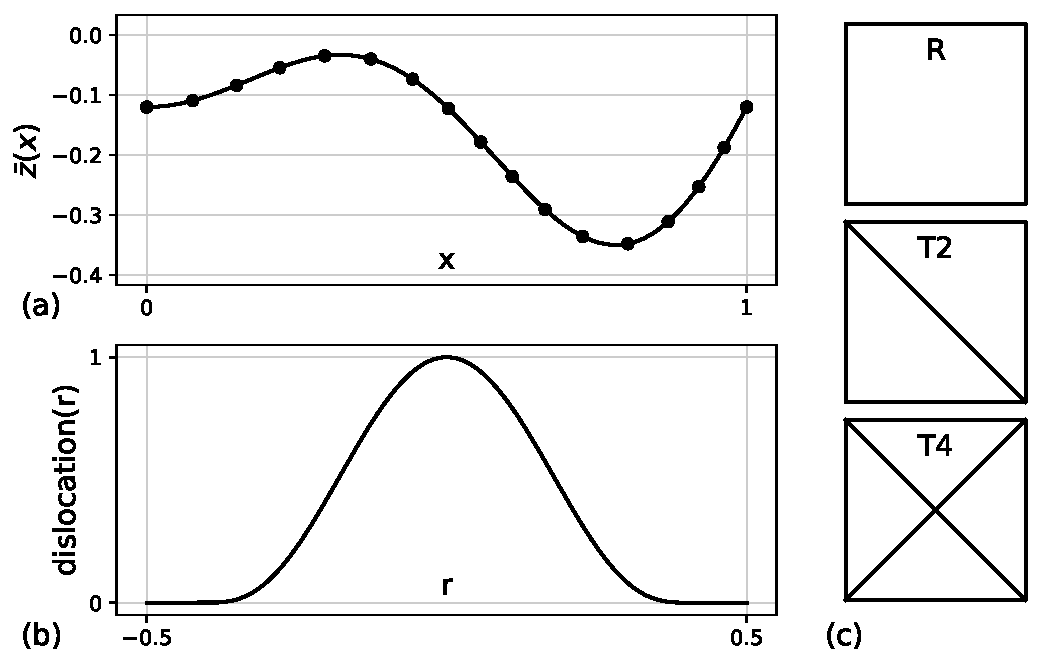
\includegraphics[width=0.8\linewidth]{schematic-line-diagrams}
  \caption{
    (a) 1D curve that is extruded into the page to make the 2D curved fracture surface.
    (b) Dislocation shape.
    (c) Three tessellation patterns based on decomposition of a rectangle.
  }
  \label{fig:problem}
\end{figure}

\begin{figure}[tb]
  \centering
  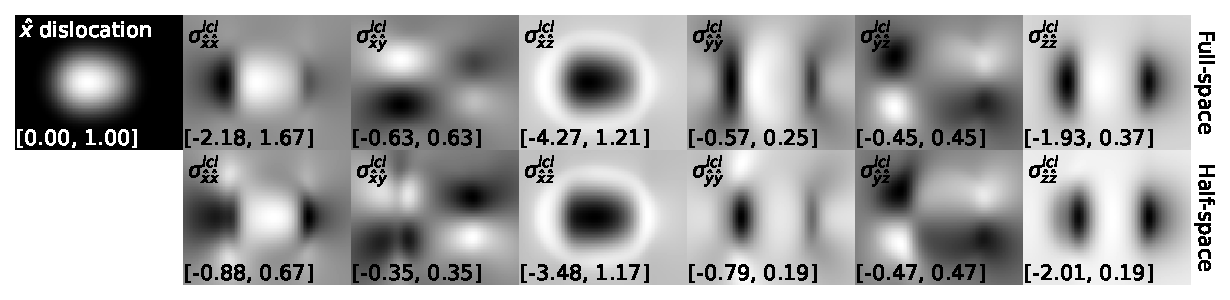
\includegraphics[width=1\linewidth]{example-soln-save}
  \caption{
    Stress components resulting from an $\hat{x}$-direction dislocation.
    Each image's $x$-axis is arc length along the 1D curve shown in Fig.~\ref{fig:problem}(a).
    Thus, the dislocation shape, based on Fig.~\ref{fig:problem}(b),
    is not circularly symmetric.
    Bracketed pairs of numbers provide the minimum (dark) and maximum (light) values.
  }
  \label{fig:solution}
\end{figure}

\begin{figure}[tb]
  \centering
  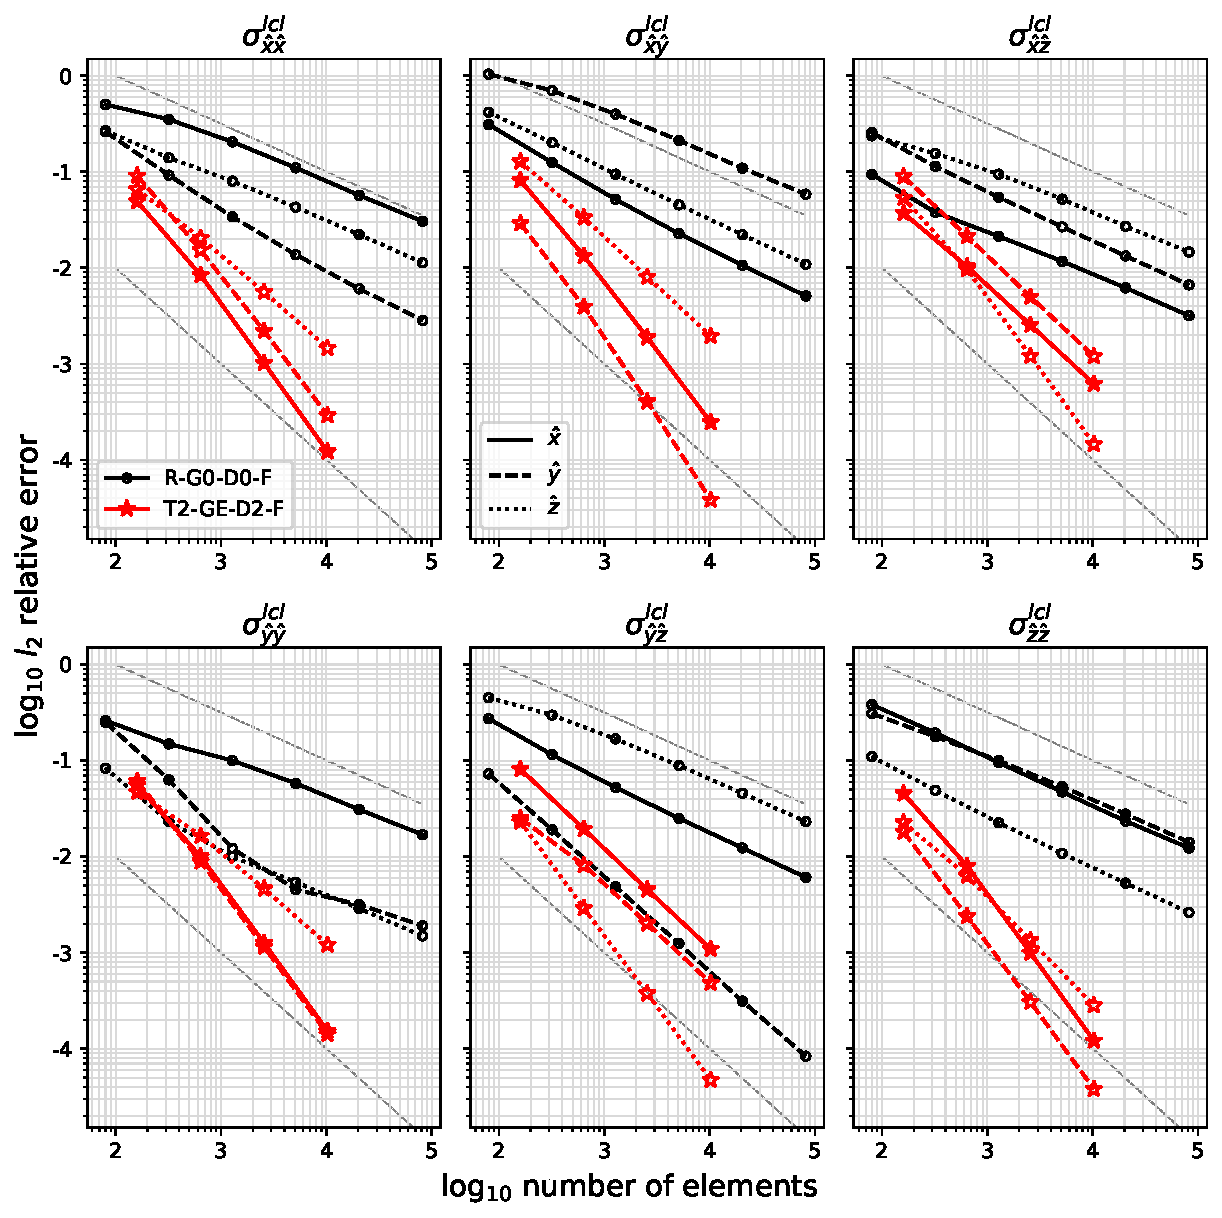
\includegraphics[width=1\linewidth]{conv-072425-basic-f}
  \caption{
    Convergence plots for components of stress using
    the reference method based on Okada's solution for flat rectangles (R-G0-D0)
    and the CSFP method with exact fracture shape and quadratic dislocation (T2-GE-D2),
    for the full-space problem.
    Thin lines are first-order and second-order convergence curves.}
  \label{fig:acc-basic-f}
\end{figure}
\begin{figure}[tb]
  \centering
  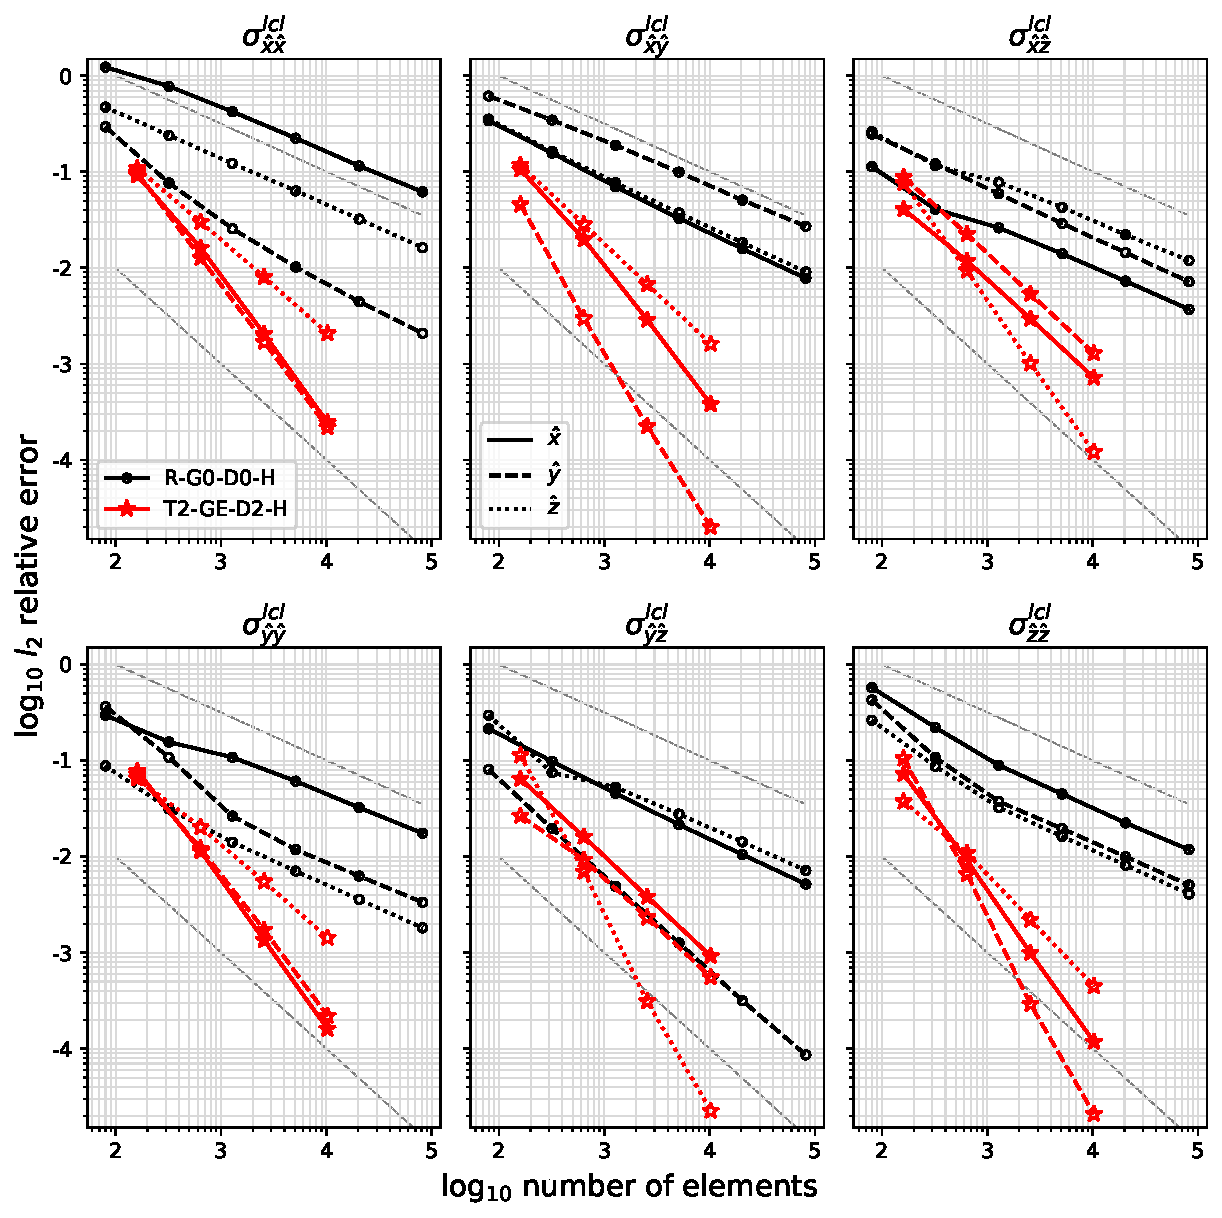
\includegraphics[width=1\linewidth]{conv-072425-basic-h}
  \caption{
    Same as Fig.~\ref{fig:acc-basic-f} but for the half-space problem.
  }
  \label{fig:acc-basic-h}
\end{figure}
\begin{figure}[tbh]
  \centering
  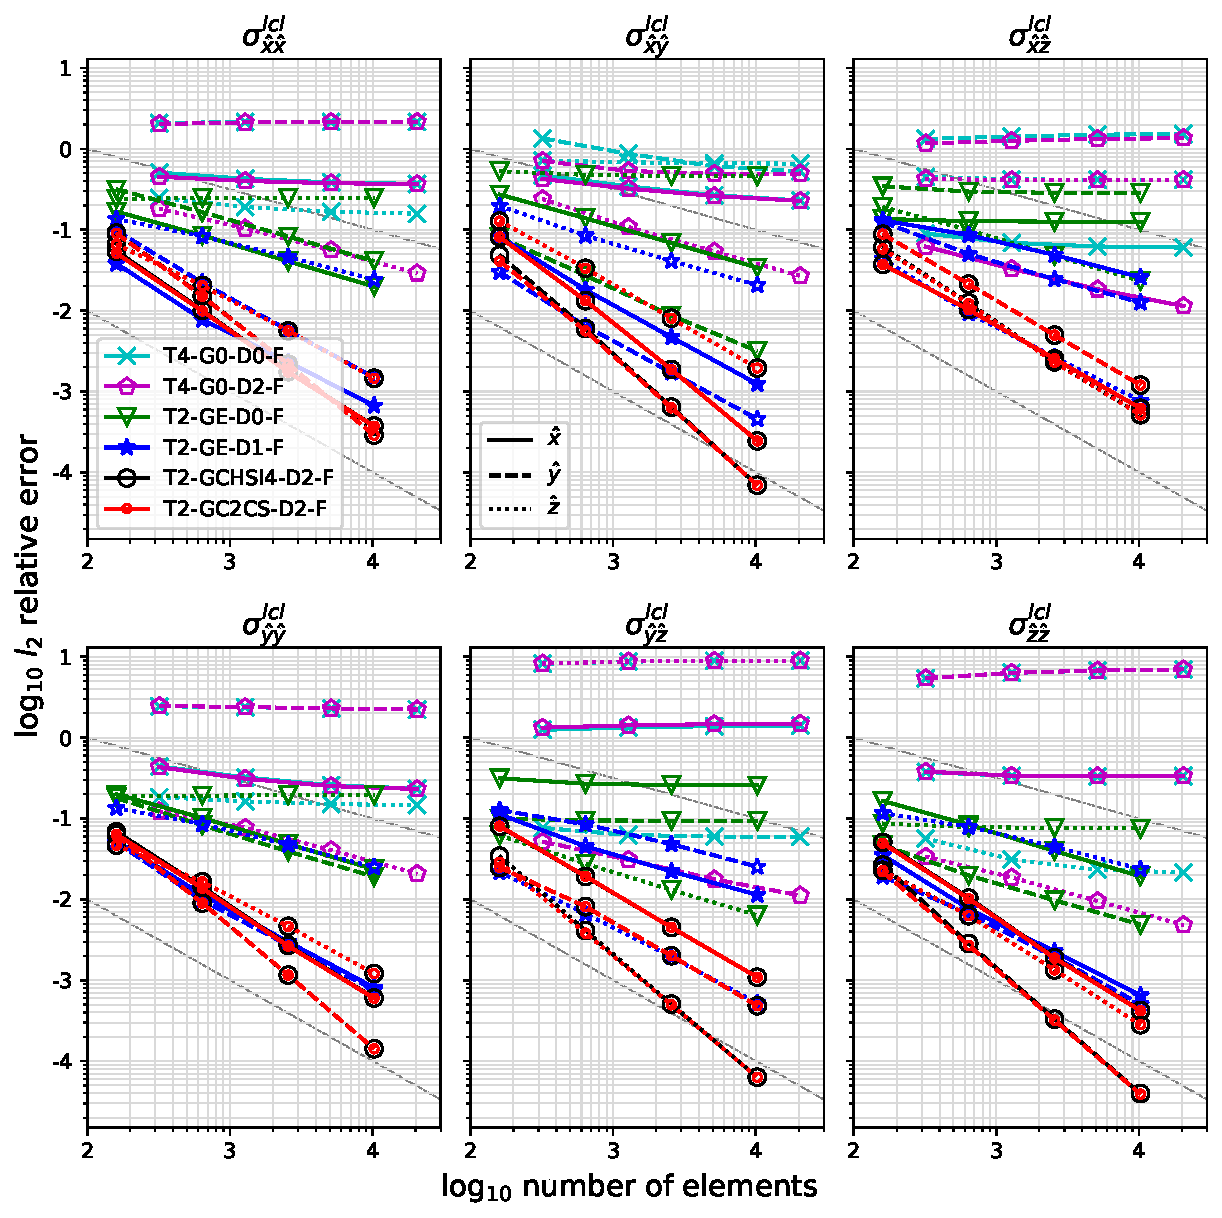
\includegraphics[width=1\linewidth]{conv-072425-necessity}
  \caption{
    Convergence plots for discretization variants.
  }
  \label{fig:acc-necessity}
\end{figure}

This section demonstrates use of our approximations to
the self- and other-interaction integrals \eqref{eq:main}
in elastic full- and half-spaces.
As a reference method, we use a discretization based on the Okada solution to the interaction integral
for a flat rectangle with constant dislocation \citep{okada1992internal}.
Because flat rectangular elements cannot cover general curved surfaces without gaps and overlaps,
we focus on a symmetry case where a rectangular tessellation is an effective approximation:
a one-dimensional curve extruded to form a two-dimensional surface.
We demonstrate our method using curved-triangle tessellations.
We also show results for flat-triangle tessellations
to demonstrate that these in general cannot be used.
All aspects of our test problem are designed to be as simple as possible
to demonstrate our key points.
In particular, the triangle tessellations are not efficient tessellations of the fracture;
curved rectangles likely would be the most efficient,
but these would hide aspects of our key points.
We examine several discretizations and, thus,
use a naming scheme to identify methods.

\subsection{Problem setup} \label{sec:problem-setup}

Figure \ref{fig:problem} shows the problem setup:
the fracture surface, the dislocation, and the tessellation types.
Figure \ref{fig:problem}(a) plots the one-dimensional curve
$\bar{z}(x) = 0.3 \ x \sin(2 \pi x) - 0.12$ for $x \in [0,1]$.
This curve is then extruded in the $y$ direction,
giving the fracture surface $z(x,y) = \bar{z}(x)$ for $(x,y) \in [0,1]^2 \equiv \Pi$,
where $\Pi$ is the parameter domain for the parameterized surface.
Convergence results are insensitive to the particular curve,
as long as the curve is smooth.
The constant $-0.12$ is chosen
to make the influence of the half-space terms significant but not dominant.
Rectangles tessellate the fracture surface.
The rectangles have uniform length in the $y$ direction.
In the $x$--$z$ plane of the curve, the spacing between element boundaries is constant in arc length.
The dots in Fig.~\ref{fig:problem}(a) show an example of this latter spacing scheme.

We use a local coordinate system (LCS) in which
$\uvec{y}$ is parallel to the $y$ direction,
$\uvec{x}$ is tangent to the physical element's surface and orthogonal to $\uvec{y}$,
and $\uvec{z}$ is normal to the element's surface.

Figure \ref{fig:problem}(b) shows the test dislocation shape:
$(1 - (2 r/b)^2)^3$ for $r \le b/2$, 0 otherwise.
In convergence tests,
$r = \sqrt{(x - 1/2)^2 + (y - 1/2)^2}$,
$b = 4/5$,
and the tangent $\uvec{x}$- and $\uvec{y}$-direction and opening $\uvec{z}$-direction
dislocations are considered separately.
Our value of $b$ makes the dislocation zero near the domain's boundary,
making the convergence curves independent of the treatment of the boundary,
which is not our focus.
While the dislocation shape is circularly symmetric in the $x$--$y$ plane,
its projection onto the fracture surface is not.

Figure \ref{fig:problem}(c) shows the three tessellation patterns we use
and their symbols in the naming scheme: a rectangle and two triangulations of the rectangle.
The midpoint of the four-triangle rectangle is found by
projecting the flat rectangle's midpoint in the $z$ direction onto the fracture surface.
This is an example of where simplicity is chosen over producing a higher-quality tessellation,
which might choose the center using the surface's arc length.
Each element in the tessellation has associated parameter polygon and physical element,
with a smooth map between the two.

There are three surface types: flat (``G0'' in discretization names), exact (``GE''),
and a set of high-order approximations of the exact surface.
This latter set is used to study the effect of approximating the surface,
but its utility is restricted to just extruded surfaces
and, thus, is not a general method.
Future work will study efficient, general, sufficiently smooth approximations for general surfaces.
In this section, the method is a cubic spline interpolant over the one-dimensional curve $\bar{z}(x)$.
In the $y$ direction, the surface is constant.
The nodal values are always exact.
We show results for three variations.
The first two are based on the cubic Hermite spline.
This spline requires nodal values and derivatives.
The derivatives must be estimated, and we use two methods.
For each node,
the first uses a quadratic interpolant over the three-node neighborhood (``GCHSI2''),
and the second uses a quartic interpolant over the five-node neighborhood (``GCHSI4'').
The first derivative of an interpolant provides the derivative estimate at the node.
The final variation is the global $C^2$ cubic spline (``GC2CS'').
This approximation requires nodal values,
as well as derivative estimates at the domain's two end points.
For these latter we use cubic interpolants over the first and final four-node neighborhoods.

Each element has one collocation point corresponding to the parameter polygon's centroid
mapped to the physical element's surface.
Each collocation point is associated with
a dislocation 3-vector $\suplcl{\vec{d}}$
and a stress tensor $\suplcl{\mat{\sigma}}$,
each in the LCS determined by the physical element's surface normal at the collocation point.
In Sec.~\ref{sec:methods}, $\vec{d}$ is in the global coordinate system (GCS).
In applications, dislocation and stress are usually represented in local coordinates.
Thus, we adopt that convention here,
but we note that representing these quantities in the GCS would work, as well.

We construct up to quadratic dislocation over each triangle
and only constant dislocation over rectangular elements.
Dislocation order is denoted ``D$n$'' for $n=0,1,2$ in method names.
Consider an element, the \emph{main} element.
Its neighborhood includes itself and those elements sharing at least one of its nodes.
Each element has a collocation point.
Each collocation point in the neighborhood
is orthogonally projected onto the plane tangent to the main element's collocation point.
A polynomial of degree $n$ is fit in a least-squares sense to each $\suplcl{d}_i$,
constrained to pass through the main element's value.
Other methods of reconstruction are possible,
but this approach is reasonable and simple.
If $n=0$, this reconstruction reduces to a constant dislocation.
To compute the coefficients of the DDM operator in the D2 case,
there are 108 interaction integrals per element--point pair:
six basis functions for a two-dimensional quadratic polynomial,
three dislocation components,
and six independent components in the symmetric stress tensor.

We show results for both the elastic full-space (``F'') and half-space (``H'').
Implementing the half-space image terms in our approach is simple.
In addition, the well-behaved half-space terms can hide issues in the singular full-space integrals.
Thus, we show half-space results in only one case.

Figure \ref{fig:solution} shows stress distributions
in the LCS for an $\hat{x}$-direction dislocation in full- and half-spaces
using the test fracture and dislocation shapes.

Results are shown as convergence plots.
Each figure shows a plot for each stress component in the LCS.
Each plot shows data for multiple discretizations
and the three dislocation components in the LCS.
The line marker style corresponds to the discretization;
the line pattern, to the dislocation component.
The line color also corresponds to the discretization
for convenience when viewing the figure in color,
but note that the color is redundant with the marker style.
The $x$-axis is $\log_{10}$ of the number of elements.
The $y$-axis is $\log_{10}$ of the $l_2$ relative error.
Two thin, dotted lines show first-order and second-order convergence curves.
Refinement is uniform in the $\uvec{x}$- and $\uvec{y}$-directions.

The reference solution must be computed numerically at high accuracy.
Consider a point $\vec{p} \in \Pi$ at which this solution is sought.
$\Pi$ is divided into an 11$\times$11 grid of rectangles.
One rectangle is centered on $\vec{p}$
except when the point is near a boundary.
The other rectangles are adjusted to roughly uniformly tessellate $\Pi$.
The exact fracture shape and dislocation and very accurate quadrature
are used to compute the stress components,
using the CSFP method, at $\vec{p}$.
This procedure is repeated for each of a discretization's collocation points.
The reported error is then the element-area-weighted $l_2$ norm of
the difference between the discretization's approximate solution
and the reference solution at the collocation points
divided by the norm of the reference solution.

Because the procedure to compute the reference solution uses
the same fundamental algorithms and software as most of the discretizations,
we must consider how correctness of these is established.
The R-G0-D0 method uses the Okada solution and code for rectangular dislocations \citep{okada1992internal}.
This converges to the reference solution,
implying the reference solution is correct to at least the accuracy the R-G0-D0 method achieves.
Tests using a flat fracture, not shown, establish correctness to higher levels of accuracy
because the R-G0-D0 method converges at a higher rate for a flat fracture than a curved one.
Finally, as part of automated unit tests,
we compare the CSFP method against the Okada code
for a single constant-dislocation, full- or half-space, flat rectangle,
establishing correctness to approximately ten digits or more in this case.

Problem symmetries let us reduce the number of unique integrals
over the whole tessellation substantially.
On a ten-year-old workstation and using one thread,
each T2-GE-D2-F convergence curve is computed in 5 minutes;
each T2-GE-D2-H curve, 23 minutes.

At the highest resolution used in the convergence study,
the R-G0-D0 method has spikes of numerical noise in some components of the stress tensor.
These result from a combination of an accuracy limit in the element Green's function calculations
and cancellation error when transforming $\mat{\sigma}$ from global to receiver-local coordinates.
We decided to keep these final points, however,
because the numerical error is limited sufficiently such that
the rightmost part of the convergence curves are not visibly affected.
Again for the R-G0-D0 method,
the $\uvec{y}$-dislocation $\suplcl{\sigma}_{\uvec{y}\uvec{y}}$ curve bends at lower resolution due to intrinsic error in the method,
not due to this numerical noise.

\subsection{Results}

\begin{table}
\centering
\begin{tabular}{r|p{0.6\linewidth}|l}
R-G0-D0 & Constant dislocation over flat rectangular elements & OOA 1 \\
\hline
T2-GE-D2 & Quadratic dislocation over exactly curved triangles & OOA 2 \\
\hline
T2-GCHSI2-D2 & Quadratic dislocation over triangles with cubic Hermite spline geometry, quadratic interpolants for derivatives & OOA 1 \\
\hline
T2-GCHSI4-D2 & Quadratic dislocation over triangles with cubic Hermite spline geometry, quartic interpolants for derivatives & OOA 2 \\
\hline
T2-GC2CS-D2 & Quadratic dislocation over triangles with global $C^2$ cubic spline geometry & OOA 2 \\
\hline
T2-GE-D0 & Constant dislocation over exactly curved triangles & nonconvergent  \\
\hline
T2-GE-D1 & Linear dislocation over exactly curved triangles & OOA 1  \\
\hline
T4-G0-D0 & Constant dislocation over flat triangles & nonconvergent \\
\hline
T4-G0-D2 & Quadratic dislocation over flat triangles & nonconvergent
\end{tabular}
\caption{
  Summary of methods, excluding the full-space (``-F'') and half-space (``-H'') suffixes.
  Results are invariant to these spaces.
  The worst order of accuracy (OOA) among the 18 stress-dislocation components is listed.
}
\label{tbl:nomen}
\end{table}

Table \ref{tbl:nomen} summarizes the discretizations methods, names, and results
that we discuss in this section.

Figure \ref{fig:acc-basic-f} compares the basic high-order method,
a triangle tessellation with exact fracture geometry
and a quadratic representation of dislocation,
with R-G0-D0 in the full-space problem.
T2-GE-D2 provides at least second-order accurate convergence
for all dislocation directions and stress components.
R-G0-D0 provides first or slightly worse convergence order
in most components, with one case of second-order convergence.
Figure \ref{fig:acc-basic-h} shows the same comparison for the half-space problem.
Recall that R-G0-D0 can be used only because the fracture's
shape is an extruded 1D curve.
Fractures having general shapes cannot be tessellated by flat rectangles.

Figure \ref{fig:acc-necessity} explores
several discretization variants.
First, exact geometry can be reduced to the GCHSI4 and GC2CS approximations
while maintaining at least second-order accuracy,
as the T2-GCHSI4-D2 and T2-GC2CS-D2 curves show.
The GCHSI2 geometry approximation, not shown,
provides only first-order accuracy in some components.
Thus, $C^1$ continuity is sufficient for second-order convergence in the case of an extruded grid,
but the derivative estimates must be sufficiently accurate.
Alternatively, nodal data combined with a $C^2$ approximation is also sufficient.

The T4-G0-D0 discretization, flat triangles with constant dislocation,
is nonconvergent in every component.
Quadratic representation of dislocation over flat triangles, T4-G0-D2, can fix only a few components.
Thus, for collocation DDM discretizations of generally curved fractures,
it is necessary to use curved elements.

The T2-GE-D0 discretization, exact geometry with constant dislocation,
is convergent in some but not all components,
showing that high-order approximation of dislocation is also necessary.
T2-GE-D1 indicates that first-order representation is sufficient for convergence.

% this checks the following statement:
% for tc in 10 20 21; do OMP_NUM_THREADS=4 ./squirrel/testmain ct_we_zx testcase=$tc,nres=4,srfrecon=0,dislocorder=1; done
We omit plots for flat fractures, but in this case,
a general triangular tessellation, here T2, and constant dislocation again lead to
nonconvergence in all nonzero components in the full-space problem.
Thus, for general tessellations, at least linear dislocation is necessary.
Recall that for flat elements and high-order dislocation,
the CSFP method is likely unnecessary;
standard closed-form methods are likely possible.
Thus, a closed-form interaction integral supporting at least linear dislocation
can be used to discretize flat fractures with general, nonuniform polygons.

\section{Conclusions} \label{sec:conclusions}

We presented the circular-sector finite-part method to compute the self-interaction integral
in collocation DDM discretizations of curved fractures.
Such discretizations can be used, for example,
as part of a quasi-dynamic earthquake simulator modeling curved fractures.
We presented numerical results in which
we used a curved fracture with sufficient symmetry
to permit comparison of solutions from our method
with those based on the code of \citet{okada1992internal}.
Finally, we showed shortcomings of other potential methods and,
thus, the necessity in general of both
(1) curved elements and a new method to compute the self-interaction integral over such an element and
(2) high-order representation of dislocation.

A general-purpose DDM discretization method and software library
that uses this method must provide the smoothness properties described in Section~\ref{sec:problem-setup}.
It should support both simple closed-form specification of fracture geometry
and sufficiently smooth reconstruction of fracture geometry data.
The DDM simulation grid should be distinct from the geometric reconstruction,
since the simulation grid's local element size must scale with the crack nucleation length scale,
while the geometric reconstruction should grow in complexity with the fracture shape.
It should provide boundary conditions for the fault.
Finally, it should use H-matrix approximation, e.g. \citet{bradley2014software},
to compress the BEM matrices constructed using the methods in this document.

\section*{Computer code availability}

The open-source (BSD 3-Clause License) C++ library Woodland \citep{woodland-software}
is available at \url{https://github.com/sandialabs/woodland}.

\appendix
\section{Evaluating $F(r,\theta_1,\theta_2)$ at $r=0$} \label{sec:Fr0}

To sample $r \in [0, \rmax]$, i.e., all the way to 0 rather than to $\varepsilon \rmax$,
we must compute $F(r,\theta_1,\theta_2)$ at $r=0$.
The advantage of being able to do this is that $\bar{p}(r)$ is then fully an interpolant;
no extrapolation is needed.
In practice, we find no meaningful difference in the computed integrals,
but we provide this appendix for completeness.
Furthermore, since we can carry out this calculation in our code,
we do so in practice.

For this calculation, we need more detailed forms of \eqref{eq:general-integral} and \eqref{eq:general-case}.
First, we change the arguments to $\sigma_{ij}$.
Originally, we wrote them as $(\vec{x}, \vec{y}(\vec{\alpha}), \uvec{n}(\vec{\alpha}), \vec{d}(\vec{\alpha}))$,
where $\vec{x}$ is the receiver and $\vec{y}$ is the source.
The Green's function uses the direction $\vec{x} - \vec{y}$,
not $\vec{x}$ and $\vec{y}$ individually.
In addition, now we must consider the case $\vec{y} = \vec{x}$.
Let $\uvec{v}$ be the unit direction vector from $\vec{y}$ to $\vec{x}$
and $R(\vec{x},\vec{y})$ be the distance $\|\vec{x}-\vec{y}\|_2$.
Thus, for clarity, $\vec{x}-\vec{y} = R(\vec{x},\vec{y}) \uvec{v}$.
Then the Green's function can be written in terms of these arguments:
$(R, \uvec{v}(\vec{\alpha}), \uvec{n}(\vec{\alpha}), \vec{d}(\vec{\alpha}))$.
$\uvec{v}$ has significance even when $R=0$.
This modification only trivially affects a caller's point Green's function subroutine.

Second, we ask that that the caller organize the subroutine such that $R^{-3}$ factors out of the expressions.
If requested, the subroutine should return $\lim_{R \rightarrow 0} \sigma_{ij} R^3$,
which is the smooth, nonsingular function remaining when $R^{-3}$ is factored out and dropped.

Third, with these modifications to the caller's point Green's function,
we can organize the calculation of $F(r,\theta_1,\theta_2)$ when $r = 0$ as follows.
Now we write the integrand of \eqref{eq:general-integral} as
\begin{linenomath}\begin{equation*}
  \sigma_{ij}(R, \uvec{v}(\vec{\alpha}), \uvec{n}(\vec{\alpha}), \vec{d}(\vec{\alpha})) \
  \sqrt{\mathrm{det}(\vec{y}_{\vec{\alpha}}(\vec{\alpha})^T \vec{y}_{\vec{\alpha}}(\vec{\alpha}))} \
  | \mathrm{det}(\vec{\alpha}_{(r,\theta)}) |.
\end{equation*}\end{linenomath}
As in \eqref{eq:general-case}, we use radial coordinates centered at the receiver.
Thus, $\sigma_{ij}$ can be written as
\begin{linenomath}\begin{equation*}
  \sigma_{ij}(R, \uvec{v}(\vec{\alpha}), \uvec{n}(\vec{\alpha}), \vec{d}(\vec{\alpha})) =
  \frac{\hat{k}(r,\theta)}{R(r,\theta)^3}.
\end{equation*}\end{linenomath}
We also combine the area elements into one:
\begin{linenomath}\begin{equation*}
  \sqrt{\mathrm{det}(\vec{y}_{\vec{\alpha}}(\vec{\alpha})^T \vec{y}_{\vec{\alpha}}(\vec{\alpha}))} \
  | \mathrm{det}(\vec{\alpha}_{(r,\theta)}) |
  = \sqrt{\mathrm{det}(J(r,\theta)^T J(r,\theta))}.
\end{equation*}\end{linenomath}
$J$ is the Jacobian matrix of the map $\vec{y}(\vec{\alpha}(r,\theta))$ with respect to $(r,\theta)$.
Finally, we combine the smooth, nonsingular factors into one:
\begin{linenomath}\begin{equation*}
  \hat{f}(r,\theta) \equiv \hat{k}(r,\theta) \sqrt{\mathrm{det}(J(r,\theta)^T J(r,\theta))}.
\end{equation*}\end{linenomath}
For a smooth, nonsingular parameterization of a smooth surface,
\begin{linenomath}\begin{equation*}
  \lim_{r \rightarrow 0} \frac{r}{R(r,\theta)} > 0.
\end{equation*}\end{linenomath}
Then we can write
\begin{linenomath}\begin{equation*}
  \frac{\hat{f}(r,\theta)}{R(r,\theta)^3}
  = \frac{\hat{f}(r,\theta) \, [r/R(r,\theta)]^3}{r^3}
  = \frac{f(r,\theta)}{r^3},
\end{equation*}\end{linenomath}
where $f(r,\theta) \equiv \hat{f}(r,\theta) \, [r/R(r,\theta)]^3$
is again a smooth, nonsingular function,
yielding the form of the integrand used in \eqref{eq:general-case}.

Fourth, let $\uvec{p}(\theta) \equiv (-\cos \theta, -\sin \theta)$.
$\uvec{p}$ is the unit vector in the parameter space pointing from the source to the receiver.
Then at $r=0$, $\uvec{v}(r,\theta) = J(0,\theta) \uvec{p}(\theta)$.
The caller is asked to compute
$\sigma_{ij}(0, J(0,\theta) \uvec{p}(\theta), \uvec{n}(\vec{\alpha}(0,\theta)), \vec{d}(\vec{\alpha}(0,\theta)))$,
excluding the $R^{-3}$ factor, for various values of $\theta$.
Thus, we have access to $\hat{k}(0,\theta)$ and $\hat{f}(0,\theta)$.

Finally, as in \eqref{eq:general-case},
we seek $F(r,\theta_1,\theta_2) \equiv \int_{\theta_1}^{\theta_2} f(r,\theta) \ \mathrm{d} \theta$,
now with $r=0$.
First,
\begin{linenomath}\begin{equation*}
  F(r,\theta_1,\theta_2) \equiv \int_{\theta_1}^{\theta_2} f(r,\theta) \ \mathrm{d} \theta
  = \int_{\theta_1}^{\theta_2} \hat{f}(r,\theta) \frac{r^3}{R(r,\theta)^3} \ \mathrm{d} \theta.
\end{equation*}\end{linenomath}
Second,
\begin{linenomath}\begin{align*}
  F(0,\theta_1,\theta_2)
  &= \int_{\theta_1}^{\theta_2} \lim_{r \rightarrow 0} \left( \hat{f}(r,\theta) \frac{r^3}{R(r,\theta)^3} \right) \mathrm{d} \theta \\
  &= \int_{\theta_1}^{\theta_2} \hat{f}(0,\theta) \left( \lim_{r \rightarrow 0} \frac{r}{R(r,\theta)} \right)^3 \mathrm{d} \theta.
\end{align*}\end{linenomath}
Third,
\begin{linenomath}\begin{align*}
  \lim_{r \rightarrow 0} \frac{r}{R(r,\theta)}
  &= \lim_{r \rightarrow 0} \frac{1}{R_r(r,\theta)} \\
  &= \left( \uvec{p}(\theta) \ J(0,\theta)^T J(0,\theta) \ \uvec{p}(\theta) \right)^{-\frac{1}{2}},
\end{align*}\end{linenomath}
which is smooth and nonsingular.
In summary,
\begin{linenomath}\begin{equation*}
  F(0,\theta_1,\theta_2)
  = \int_{\theta_1}^{\theta_2} \frac{\hat{f}(0,\theta)}{(\uvec{p}(\theta) \ J(0,\theta)^T J(0,\theta) \ \uvec{p}(\theta))^\frac{3}{2}} \ \mathrm{d} \theta,
\end{equation*}\end{linenomath}
which is a proper integral.

\addcontentsline{toc}{section}{References}
\bibliographystyle{plainnat}
\bibliography{references}

\end{document}
